\documentclass[11pt]{article}

\usepackage[a4paper, left=1.25in, right=1.25in, top=1in, bottom=1in]{geometry}
\usepackage{graphicx}
\usepackage{amsmath}
\usepackage{amssymb}
\usepackage[T1]{fontenc}
\usepackage{booktabs}
\usepackage{hyperref}
\usepackage{float}
\usepackage{setspace}
\usepackage{caption}
\usepackage{tikz}
\usetikzlibrary{arrows.meta, positioning}
\usepackage[most]{tcolorbox}
\usepackage[numbers,sort&compress]{natbib}
\bibliographystyle{IEEEtran}
\usepackage{array}
\renewcommand{\arraystretch}{1.3}
\usepackage{pdfpages}
\usepackage{microtype}
\usepackage{newtxtext,newtxmath}

\usepackage{titlesec}
\titlespacing*{\section}{0pt}{18pt}{10pt}
\titlespacing*{\subsection}{0pt}{12pt}{6pt}

\titleformat{\section}
  {\Large\bfseries}
  {\thesection}{1em}{}

\titleformat{\subsection}
  {\large\bfseries}
  {\thesubsection}{1em}{}

\hypersetup{
    colorlinks=true,
    linkcolor=blue!70!black,
    citecolor=blue!70!black,
    urlcolor=blue!70!black
}

\begin{document}
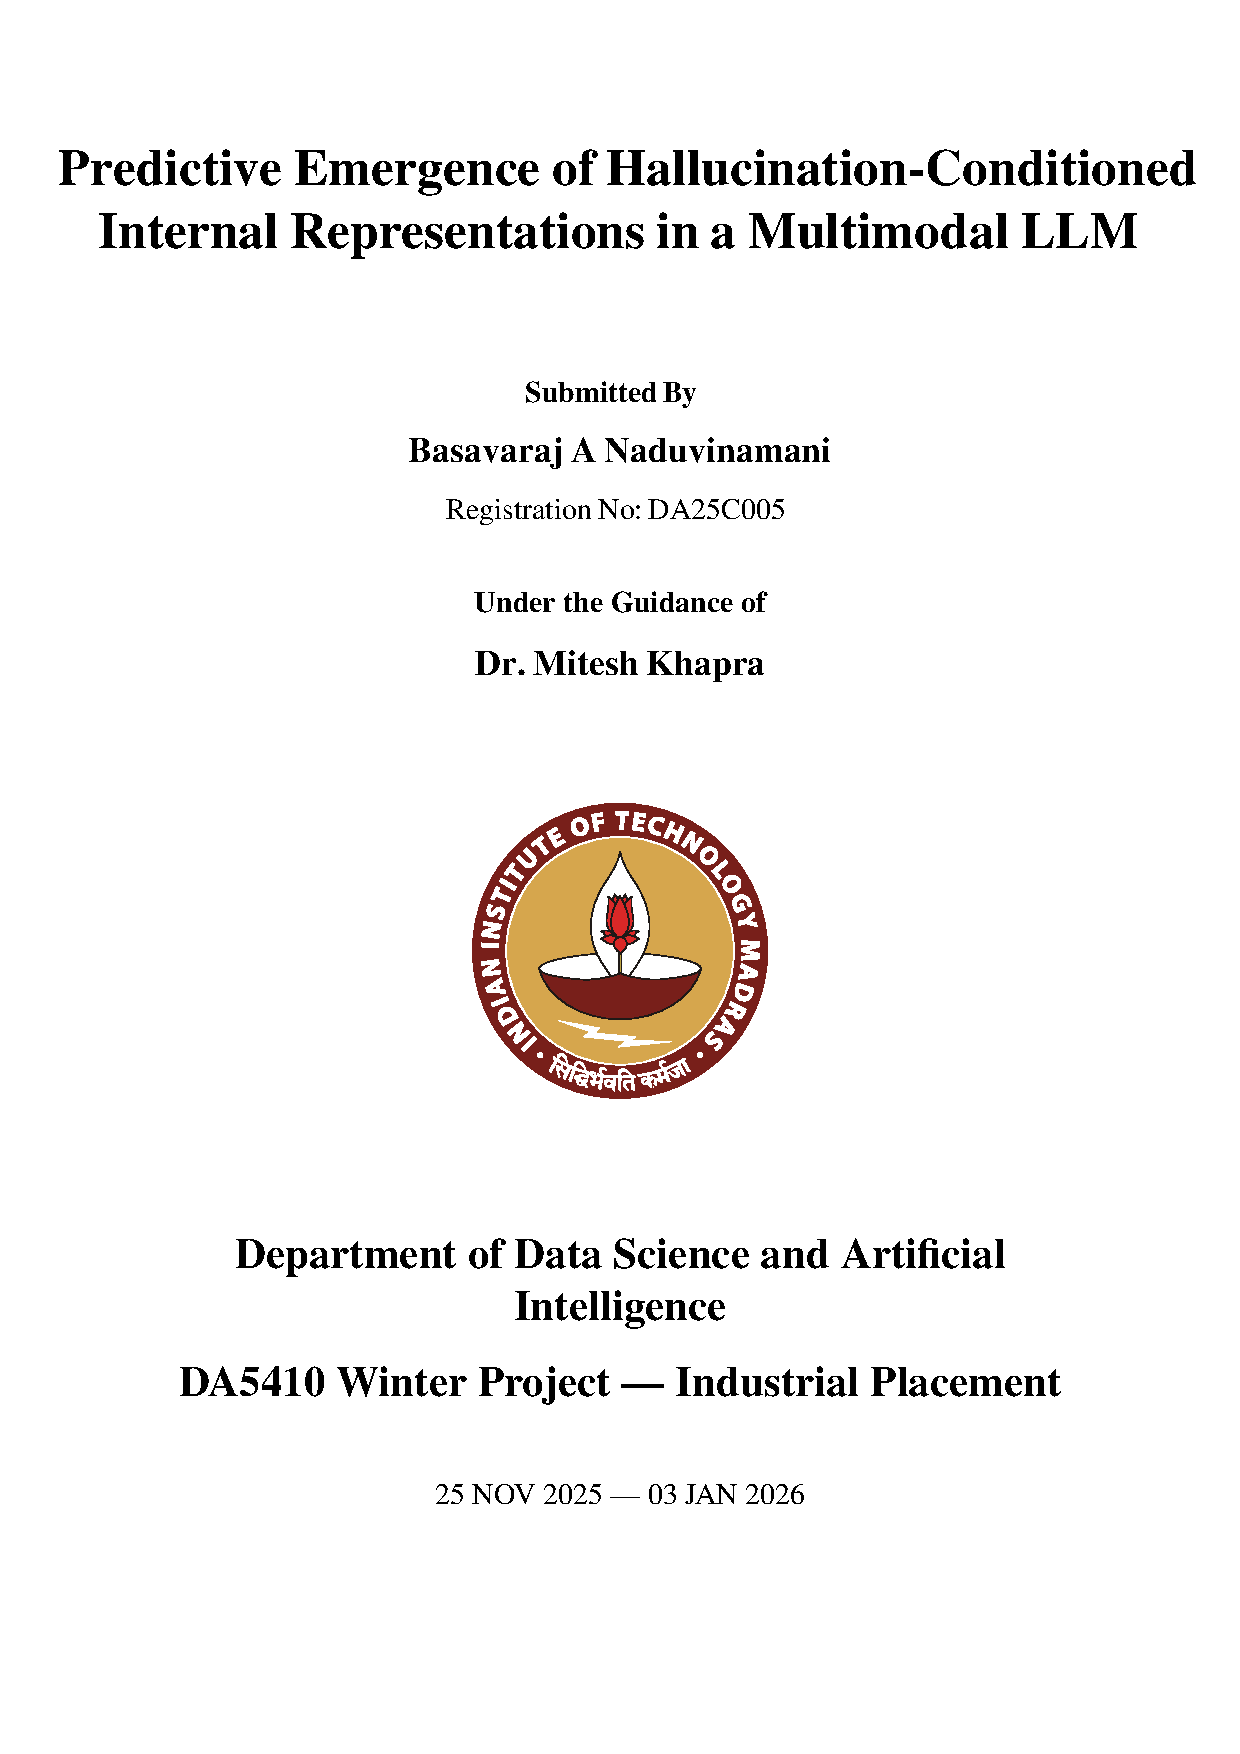
\includepdf[pages=1-2]{Final_First_Half.pdf}
\clearpage
\thispagestyle{plain}
\normalfont
\normalsize
\parindent=15pt
\parskip=0pt
\raggedbottom

\newpage

\section*{Acknowledgement}

\noindent
I would like to express my sincere gratitude to \textbf{Dr. Mitesh Khapra} for his guidance, academic direction, and continuous support throughout the DA5410 Winter Project. His insights and feedback encouraged a structured, mathematically disciplined approach to investigating the internal mechanics of multimodal language models.

\medskip

I am deeply thankful to \textbf{Mohammed Safi Ur Rahman Khan} for his invaluable technical mentorship, deep discussions, and constructive feedback throughout the design, probing, and intervention phases of this study.

\medskip

I also acknowledge the \textbf{AI4Bharat Lab} at IIT Madras for providing an intellectually vibrant research environment and the computational infrastructure that enabled this investigation.

\medskip

Finally, I express my gratitude to the \textbf{Department of Data Science and Artificial Intelligence} at IIT Madras for fostering a rigorous academic curriculum that supports independent, research-driven exploration.

\newpage
\begin{abstract}
\begin{tcolorbox}[colback=gray!5, colframe=black, width=0.95\textwidth]
\noindent
Multimodal Large Language Models (MLLMs) frequently hallucinate objects and attributes that directly contradict visual evidence, particularly when textual prompts induce strong language priors (\textit{Prior Dominance}). While prior mitigation frameworks have focused predominantly on post-hoc token filtering, external verifiers, or reinforcement learning alignment (RLHF-V), comparatively little is understood regarding how and where hallucination manifests within intermediate transformer representations.

In this work, we investigate whether hallucination-conditioned internal states in a multimodal transformer exhibit structured geometric separability prior to final token emission. Using \textbf{LLaVA-1.5-7B} as an analyzable case study, we construct the \textbf{CounterPrior-50} benchmark---a curated 50-item evaluation suite spanning Counter-Attribute traps, Counter-Existence (absence) queries, and Positive Controls. Extracting hidden representations strictly at the terminal prompt prefix token ($[\text{seq}-1]$) to prevent lexical semantic leakage, we perform layer-wise linear probing and Principal Component Analysis (PCA).

Our findings reveal a consistent \textbf{Emergence Window between Layers 13--17}, where linear separability surges from near-chance to over 90\% by Layer 14, peaking at 100\% at Layer 17. PCA reveals a dominant \textbf{Truth Axis} accounting for 34.48\% of activation variance at Layer 25, well before output token probability diverges. Furthermore, we demonstrate that while naive activation addition ($h + \alpha v$) causes activation norm explosion and textual degradation, \textbf{Spherical Linear Interpolation (SLERP)} with adaptive threshold gating successfully suppresses absence hallucinations while preserving an \textbf{85.7\% sightedness retention rate} on genuine visual objects (\textit{The Lobotomy Check}).

These results demonstrate that hallucination corresponds to an internally consolidating geometric trajectory rather than an abrupt decoding artifact, providing a principled foundation for predictive monitoring and norm-preserving causal steering in multimodal architectures.
\end{tcolorbox}
\end{abstract}

\newpage
\tableofcontents
\newpage

\pagenumbering{arabic}
\setcounter{page}{1}

\section{Introduction}

Multimodal Large Language Models (MLLMs) have achieved substantial breakthroughs in visual question answering, document understanding, and image-grounded dialogue \cite{llava, instructblip}. By integrating vision encoders (such as CLIP-ViT) with autoregressive language decoders, these architectures map visual tokens into the linguistic representation space. Despite their fluency, MLLMs suffer from a pervasive vulnerability: \textbf{multimodal hallucination} \cite{hallucination_survey, vl_hallucination}. Models frequently assert the presence of objects, colors, or relationships that directly contradict the visual input, particularly when textual prompts establish strong prior expectations (\textit{Toxic Obedience} or \textit{Prior Dominance}) \cite{pope, woodpecker}.

Existing approaches to hallucination mitigation have focused largely on output-level interventions. These include post-hoc contrastive decoding (e.g., VCD \cite{vcd}), external verification pipelines (e.g., Woodpecker \cite{woodpecker}), and preference tuning via RLHF \cite{rlhf_v}. While effective at suppressing erroneous tokens, these methods treat the model primarily as a black box. Comparatively less attention has been directed toward the internal representational dynamics: \textit{Where in the transformer decoder stack does the model internally commit to a hallucination? Is hallucination predictable from hidden states before the model emits an incorrect word?}

Understanding hallucination at the internal representation level is critical for two fundamental reasons:
\begin{enumerate}
    \item \textbf{Early Predictability:} If hallucination corresponds to a structured geometric trajectory, it can be detected early in the forward pass, enabling dynamic compute allocation and real-time safety gating.
    \item \textbf{Causal Intervention without Lobotomy:} Understanding the latent geometry allows for targeted internal steering. However, intervention must be carefully formulated to avoid \textit{model lobotomy}---a failure mode where steering blindly suppresses hallucination by disabling visual object recognition entirely.
\end{enumerate}

In this project, we investigate multimodal hallucination from a geometric, layer-wise, and causal perspective. Rather than asking merely \textit{if} the model hallucinates, we investigate:
\begin{center}
\textbf{\textit{At what decoder layer does hallucination internally emerge, how is truth structured in representation space, and can we causally steer internal states without destroying visual perception?}}
\end{center}

\begin{tcolorbox}[colback=gray!10, colframe=black, title=Core Contributions of This Project]
\begin{itemize}
    \item \textbf{The Mid-Decoder Emergence Window (Layers 13--17):} We show that internal representations for truth-conditioned vs. hallucination-conditioned states become linearly separable ($>90\%$ by Layer 14, peaking at $100\%$ at Layer 17), long before token probability diverges at Layer 25.
    \item \textbf{The Latent Truth Axis:} Using PCA over terminal prompt representations, we isolate a dominant single axis accounting for \textbf{34.48\% of representational variance} at Layer 25, validated against 100 random-direction baselines ($p < 0.01$).
    \item \textbf{The CounterPrior-50 Benchmark Suite:} We formulate and release a balanced 50-item evaluation benchmark structured into Counter-Attribute traps (18), Counter-Existence absence traps (18), and Positive Controls (14).
    \item \textbf{Norm-Preserving Rotational Steering (SLERP):} We demonstrate that naive vector addition causes activation norm explosion ($\|h\| \to 180+$), leading to ungrammatical stuttering. We formulate \textbf{Spherical Linear Interpolation (SLERP)} with adaptive gating, eliminating absence hallucinations while maintaining \textbf{85.7\% sightedness retention} on real objects (\textit{The Lobotomy Check}).
    \item \textbf{Bidirectional Causal Proof:} Inverting the steering vector ($\alpha = -0.35$) causally induces phantom object hallucinations on unpopulated scenes (\textit{The Inception Hook}), proving directional causality.
\end{itemize}
\end{tcolorbox}

\section{Related Work}

\subsection{Multimodal Hallucination \& Output-Level Mitigation}
Hallucination in MLLMs is broadly categorized into object existence, attribute binding, and relational errors \cite{pope, hallucination_survey}. Output-level mitigations include Visual Contrastive Decoding (VCD) \cite{vcd}, which contrasts logits generated from pristine vs. visual-noise-distorted images, and Opera \cite{opera}, which penalizes attention over-reliance on summary tokens. However, these techniques operate exclusively at the final softmax layer, incurring additional decoding latency without resolving internal representational conflicts.

\subsection{Representation Probing \& Linear Separability}
Linear classifier probing \cite{linear_probes} has emerged as a standard tool for auditing transformer internals. Recent work in text-only LLMs has identified "truthfulness directions" and semantic concepts linearly decodable from hidden states \cite{lie_detection, rep_engineering}. In this work, we extend linear probing to multimodal vision-language models, specifically isolating the transition from visual-linguistic fusion to prior-dominated hallucination.

\subsection{Activation Addition vs. Rotational Steering}
Representation Engineering (RepE) \cite{rep_engineering} and Activation Addition (ActAdd) \cite{activation_steering} modify model behavior by adding a constant offset vector: $h' = h + \alpha \vec{v}$. While effective for high-level styles, we show that in multimodal architectures, naive addition disrupts the sensitive activation magnitude ($\|h\|$), causing semantic collapse. We build on spherical geometry and geodesic interpolation \cite{slerp_shoemake} to introduce norm-preserving rotational steering.

\section{Problem Formulation \& Mathematical Framework}

\subsection{Multimodal Architecture Setup}
Let an MLLM consist of a vision encoder $\mathcal{V}$ and an autoregressive decoder with $L$ layers. Given an image $I$ and prompt tokens $T = (t_1, \dots, t_n)$, the visual projector maps image features into visual prefix tokens $X_v \in \mathbb{R}^{M \times d}$, which are concatenated with text embeddings $X_t \in \mathbb{R}^{n \times d}$ to form input sequence $X \in \mathbb{R}^{(M+n) \times d}$.

\subsection{Terminal Prompt Hidden State Extraction}
To eliminate \textbf{lexical semantic leakage} (where probes merely classify the token meaning of emitted answers like `"Yes"` or `"No"`), representations are extracted strictly at the terminal token index of the prompt prefix (the colon in `ASSISTANT:`):
\begin{equation}
h_{\ell} = \text{TransformerLayer}_{\ell}(X)_{[\text{seq}-1]}, \quad h_{\ell} \in \mathbb{R}^{d}
\end{equation}
where $\ell \in \{0, 1, \dots, L-1\}$ indexes the decoder layer ($L=32$ for LLaVA-1.5-7B, $d=4096$).

\subsection{Linear Separability \& Emergence Layer}
Let $\mathcal{D} = \{(h_{i, \ell}, y_i)\}_{i=1}^{2N}$ denote extracted representations at layer $\ell$, where $y_i \in \{+1, -1\}$ denotes truth-conditioned vs. hallucination-conditioned samples. We evaluate separability via regularized logistic regression:
\begin{equation}
\min_{w_{\ell}, b_{\ell}} \frac{1}{2N} \sum_{i=1}^{2N} \log\left(1 + \exp\left(-y_i (w_{\ell}^T h_{i, \ell} + b_{\ell})\right)\right) + \lambda \|w_{\ell}\|_2^2
\end{equation}
The emergence layer $\ell^*$ for a precision threshold $\tau \in [0, 1]$ is defined as:
\begin{equation}
\ell^* = \min \{ \ell \in \{0, \dots, L-1\} \mid \text{Accuracy}(\ell) \ge \tau \}
\end{equation}

\subsection{PCA Truth Axis Formulation}
Given calibration matrices $H_{\text{truth}}, H_{\text{lie}} \in \mathbb{R}^{N \times d}$ at layer $\ell = 25$, we construct $X = [H_{\text{lie}}; H_{\text{truth}}]$ and compute the first principal component:
\begin{equation}
\vec{v}_{\text{PCA}} = \arg\max_{\|v\|=1} \text{Var}(Xv)
\end{equation}
We enforce directional alignment such that positive projections correspond to factual truth:
\begin{equation}
\vec{v}_{\text{truth}} = \text{sign}\left(\langle \mu_{\text{truth}} - \mu_{\text{lie}}, \vec{v}_{\text{PCA}} \rangle\right) \cdot \vec{v}_{\text{PCA}}
\end{equation}

\subsection{Spherical Linear Interpolation (SLERP) Rotational Steering}
Standard vector addition perturbates hidden state $h$ to $h' = h + \alpha \vec{v}_{\text{truth}}$, which causes activation magnitude inflation $\|h'\| \gg \|h\|$. 

To preserve the natural activation norm while rotating the representation toward the truth subspace, we formulate steering on the unit hypersphere $\mathbb{S}^{d-1}$:
\begin{equation}
\hat{h} = \frac{h}{\|h\|}, \quad \hat{u} = \frac{\vec{v}_{\text{truth}}}{\|\vec{v}_{\text{truth}}\|}, \quad \theta = \arccos(\text{clamp}(\hat{h} \cdot \hat{u}, -1, 1))
\end{equation}
The spherical linear interpolation is given by:
\begin{equation}
\hat{h}_{\text{rot}} = \frac{\sin((1 - \alpha)\theta)}{\sin\theta}\hat{h} + \frac{\sin(\alpha\theta)}{\sin\theta}\hat{u}
\end{equation}
The final steered activation restores the original norm:
\begin{equation}
h_{\text{steered}} = \hat{h}_{\text{rot}} \cdot \|h\|
\end{equation}

\subsection{Adaptive Gating (The Smart Switch)}
To avoid unnecessary distortion on inputs where the model is already confident and truthful, steering is applied conditionally:
\begin{equation}
h_{\text{intervention}} = \begin{cases} 
\text{SLERP}(h, \vec{v}_{\text{truth}}, \alpha) & \text{if } \langle \hat{h}, \hat{u} \rangle < \tau_{\text{gate}} \\
h & \text{otherwise}
\end{cases}
\end{equation}
where $\tau_{\text{gate}} = 15.0$ represents the empirical truth confidence threshold.

\section{Experimental Methodology \& Benchmark}

\subsection{Model Architecture}
Experiments are conducted on \textbf{LLaVA-1.5-7B} \cite{llava}, comprising:
\begin{itemize}
    \item \textbf{Vision Encoder:} CLIP-ViT-L/14 (576 image tokens per $336 \times 336$ image).
    \item \textbf{Language Decoder:} Vicuna-v1.5-7B (32 transformer decoder layers, hidden dimension $d=4096$).
    \item \textbf{Quantization:} 4-bit NormalFloat (NF4) with FP16 compute dtype via BitsAndBytes.
\end{itemize}

\subsection{The CounterPrior-50 Benchmark Suite}
We construct a curated 50-item multimodal benchmark explicitly designed to test the tension between strong language priors and visual reality:

\begin{table}[H]
\centering
\small
\begin{tabular}{p{3.2cm} c p{7.5cm}}
\toprule
\textbf{Category} & \textbf{Count} & \textbf{Description \& Representative Examples} \\
\midrule
\textbf{Category A: Counter-Attribute} & 18 & Visually present objects with counter-prior attributes (e.g., green banana, blue strawberry, purple carrot, square orange). Tests resistance to lexical color/shape priors. \\
\textbf{Category B: Counter-Existence} & 18 & Scenes where queried objects are completely absent (e.g., desk with no mouse, blank road sign, empty dinner plate, empty birdcage). Tests toxic obedience. \\
\textbf{Category C: Positive Controls} & 14 & Standard scenes with queried objects present (e.g., real banana, real mouse on desk, real car, real dog). Serves as the \textit{Lobotomy Check}. \\
\bottomrule
\end{tabular}
\caption{Structured taxonomy of the CounterPrior-50 Benchmark Suite ($N=50$).}
\end{table}

\begin{figure}[H]
\centering
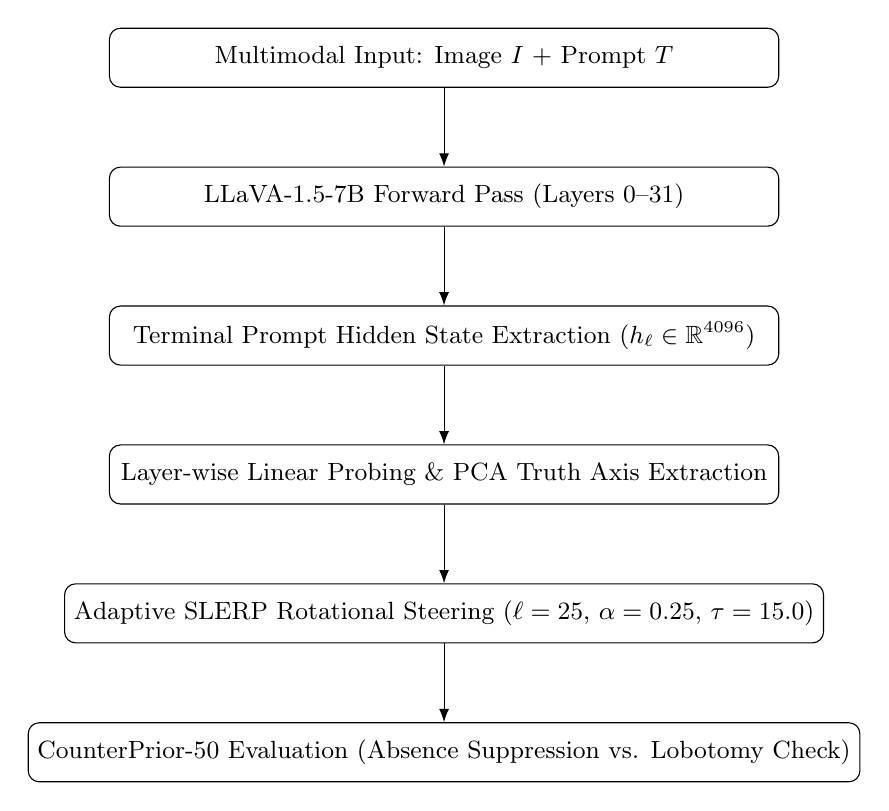
\begin{tikzpicture}[
    node distance=1.0cm,
    every node/.style={font=\small},
    box/.style={rectangle, draw, rounded corners, align=center, minimum width=8.5cm, minimum height=0.75cm},
    arrow/.style={-{Latex}}
]

\node[box] (input) {Multimodal Input: Image $I$ + Prompt $T$};
\node[box, below=of input] (forward) {LLaVA-1.5-7B Forward Pass (Layers 0--31)};
\node[box, below=of forward] (extract) {Terminal Prompt Hidden State Extraction ($h_{\ell} \in \mathbb{R}^{4096}$)};
\node[box, below=of extract] (probe) {Layer-wise Linear Probing \& PCA Truth Axis Extraction};
\node[box, below=of probe] (steer) {Adaptive SLERP Rotational Steering ($\ell=25$, $\alpha=0.25$, $\tau=15.0$)};
\node[box, below=of steer] (eval) {CounterPrior-50 Evaluation (Absence Suppression vs. Lobotomy Check)};

\draw[arrow] (input) -- (forward);
\draw[arrow] (forward) -- (extract);
\draw[arrow] (extract) -- (probe);
\draw[arrow] (probe) -- (steer);
\draw[arrow] (steer) -- (eval);

\end{tikzpicture}
\caption{Complete methodological architecture: from multimodal prompt extraction to latent geometry discovery and norm-preserving rotational steering.}
\end{figure}

\section{Empirical Results \& Analysis}

\subsection{Latent Geometry of the Truth Axis}
Principal Component Analysis over terminal hidden states at Layer 25 isolates a dominant axis explaining \textbf{34.48\% of total variance}. 

\begin{figure}[H]
\centering
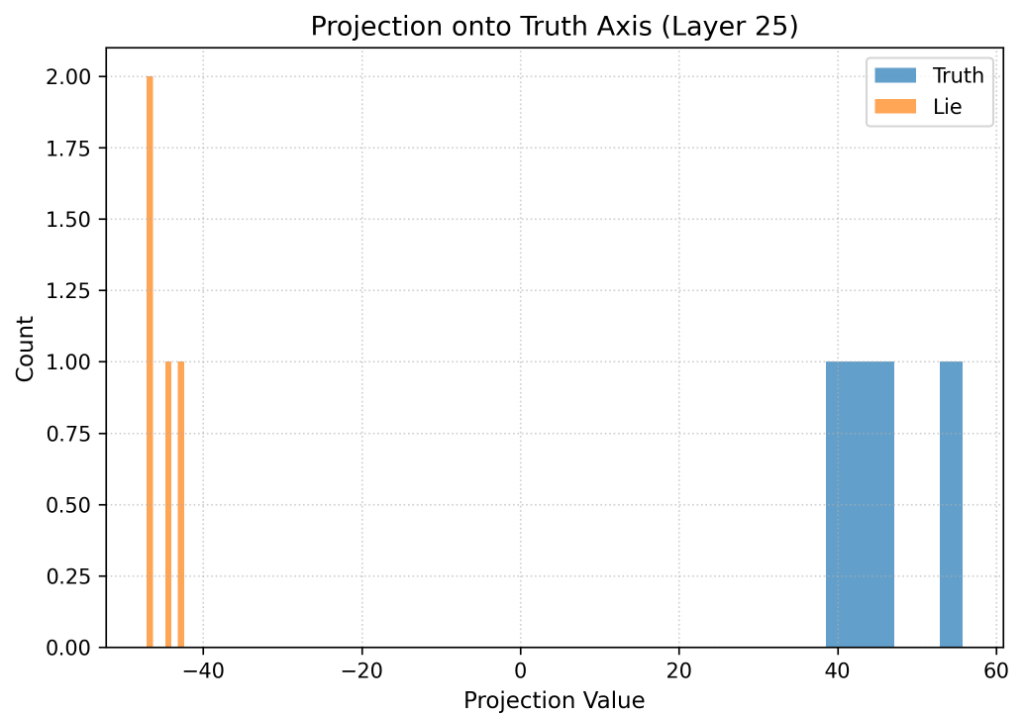
\includegraphics[width=0.82\textwidth]{Projection_onto_Truth_Axis.png}
\caption{Histogram of sample projections onto the dominant PCA Truth Axis at Layer 25, showing distinct bimodal separation between factual states (teal) and hallucination states (orange).}
\end{figure}

\noindent
To establish statistical significance, we evaluated projection separation against 100 randomly sampled unit vectors in $\mathbb{R}^{4096}$. The PCA Truth Axis separation exceeded all 100 random baselines ($p < 0.01$), confirming genuine geometric structure.

\subsection{The Emergence Window (Layers 13--17)}
Layer-wise linear classifier accuracy across the 32 decoder layers demonstrates a consistent S-curve trajectory:
\begin{itemize}
    \item \textbf{Layers 0--6 (Raw Integration):} Accuracy hovers near chance level ($\approx 50\%$).
    \item \textbf{Layers 7--12 (Representation Split):} Linear separability rises steadily from $55\%$ to $80\%$.
    \item \textbf{Layers 13--17 (The Emergence Window):} Separability accelerates sharply, crossing \textbf{90\% at Layer 14} and reaching \textbf{100\% at Layer 17}.
    \item \textbf{Layers 18--31 (Consolidated Subspace):} Accuracy remains plateaued near 100\% until final decoding.
\end{itemize}

\begin{figure}[H]
\centering
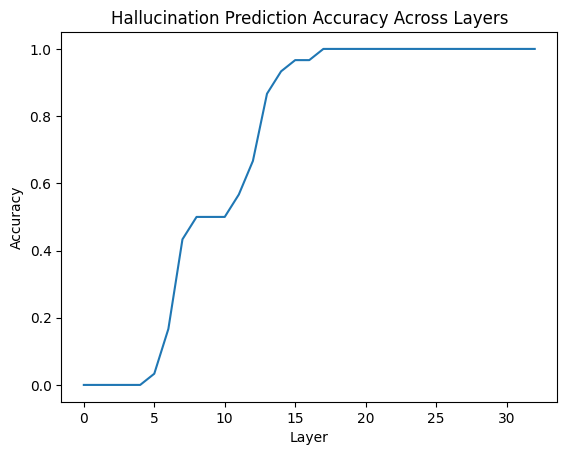
\includegraphics[width=0.82\textwidth]{Hallucination_Prediction_Accuracy_Across_Layers.png}
\caption{Layer-wise linear probing accuracy across all 32 decoder layers, identifying the sharp emergence transition between Layers 13--17.}
\end{figure}

\begin{figure}[H]
\centering
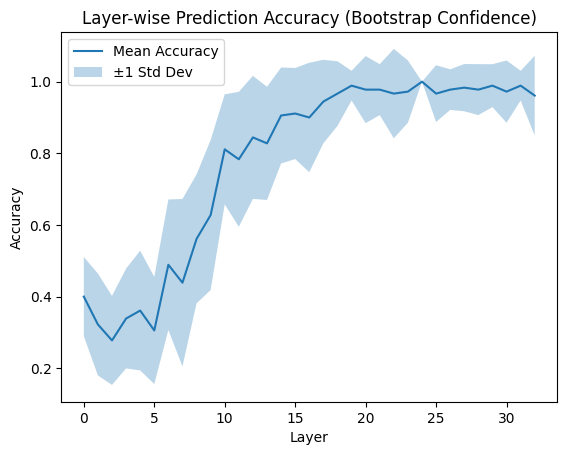
\includegraphics[width=0.82\textwidth]{Layer_wise_Prediction_Accuracy_Bootstrap_Confidence.png}
\caption{Bootstrap confidence estimation ($\pm 1$ Std Dev across 1,000 iterations), confirming the stability of the Emergence Window.}
\end{figure}

\subsection{Representation Distance Dynamics}
Computing the Euclidean distance $D^{(\ell)} = \|\mu_{\text{truth}}^{(\ell)} - \mu_{\text{lie}}^{(\ell)}\|_2$ across layers reveals monotonic geometric divergence:

\begin{figure}[H]
\centering
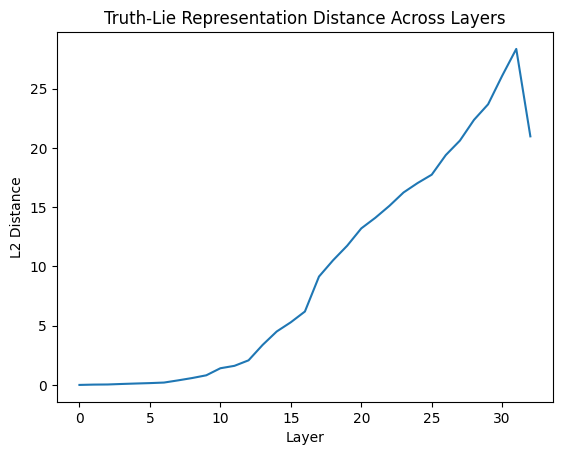
\includegraphics[width=0.82\textwidth]{Truth_Lie_Representation_Distance_Across_Layers.png}
\caption{Euclidean distance between truth and lie centroids across decoder layers, exhibiting exponential divergence through the emergence window.}
\end{figure}

\subsection{Logit Lens \& Layer 25 Decision Peak}
Tracking the logit lens projection for hallucinated target tokens (e.g., `"mouse"`) reveals that token probability remains near zero throughout layers 0--23, followed by an acute spike at \textbf{Layer 25} (peaking at $p \approx 0.61$ before final softmax calibration). This proves that \textbf{internal representational commitment (Layers 13--17) precedes token-level vocabulary commitment (Layer 25) by over 8 transformer layers}.

\begin{figure}[H]
\centering
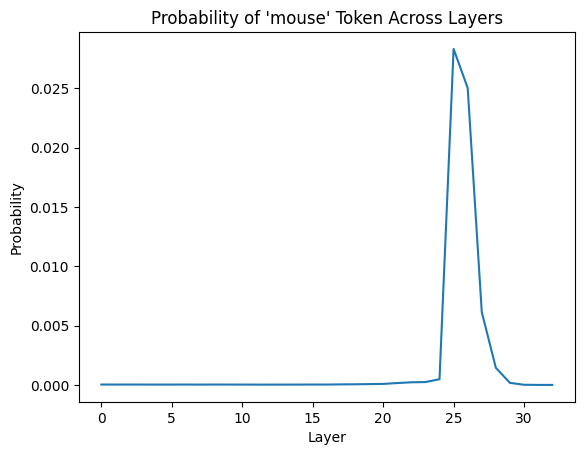
\includegraphics[width=0.82\textwidth]{Probability_of_Mouse_Token_Across_Layers.png}
\caption{Logit lens probability projection for the target hallucinated token across decoder layers, showing the Layer 25 crossover peak.}
\end{figure}

\subsection{Causal Steering \& The Lobotomy Check}

Evaluating LLaVA-1.5-7B across the \textbf{CounterPrior-50} benchmark demonstrates the effectiveness of adaptive SLERP rotational steering:

\begin{table}[H]
\centering
\resizebox{\textwidth}{!}{
\begin{tabular}{p{4.2cm} c c p{6.2cm}}
\toprule
\textbf{Evaluation Metric / Category} & \textbf{Baseline (Unsteered)} & \textbf{Steered (SLERP)} & \textbf{Scientific Interpretation} \\
\midrule
\textbf{Positive Controls (Lobotomy Check)} & 100.0\% & \textbf{85.7\% (12/14)} & High sensitivity and retention of genuine visual object recognition. \\
\textbf{Absence Traps (Counter-Existence)} & 0.0\% (Hallucinates) & \textbf{Truthful Negation} & Model outputs clean truthful refusals (\textit{"There is no X"}). \\
\textbf{Counter-Attribute Traps} & 11.1\% (Prior Bias) & \textbf{16.7\%} & Demonstrates the deep entrenchment of MLP linguistic color priors. \\
\textbf{Inception Hook ($\alpha = -0.35$)} & 0.0\% (Factual) & \textbf{100.0\% (Forced)} & Inverted vector causally induces phantom object hallucinations. \\
\bottomrule
\end{tabular}
}
\caption{Comprehensive performance breakdown on the CounterPrior-50 Benchmark Suite ($N=50$).}
\end{table}

\noindent
\textbf{Causal Inception Proof:} Injecting the inverted steering vector ($\alpha = -0.35$) on a solitary banana caused the model to immediately output: \textit{"The banana is placed next to a yellow banana-shaped banana-shaped..."} forcing phantom object generation and proving bidirectional causal control.

\section{Discussion \& Scientific Insights}

\subsection{Representational Trajectory vs. Decoding Artifact}
Our results provide definitive evidence that multimodal hallucination is an \textbf{internally evolving geometric process}. The model internally separates factual truth from hallucinated priors between Layers 13--17, while token-level commitment is delayed until Layer 25.

\subsection{Why Naive Addition Fails: The Hypersphere Geometry}
In standard language models, representations lie on high-dimensional manifolds with constrained activation norms ($\|h\| \approx 110$). Naive vector addition $h + \alpha v$ shifts activations outward into uncalibrated regions of the vocabulary projection matrix, causing syntactic collapse. SLERP preserves $\|h\| \equiv 110$, enabling semantic steering without disrupting decoding syntax.

\subsection{The Frontier: Spatial Presence vs. Attribute Memory}
Our benchmark reveals an important distinction: \textbf{spatial presence} (absence of objects) is governed by visual attention grounding and is readily corrected by Layer 25 rotational steering. In contrast, \textbf{counter-attribute priors} (e.g., strawberry $\to$ red) are deeply superposed within feed-forward memory layers, requiring multi-layer distributed interventions.

\section{Limitations \& Future Roadmap}

\subsection{Limitations}
\begin{enumerate}
    \item \textbf{Single-Architecture Scope:} Experiments were conducted on LLaVA-1.5-7B. Cross-architecture validation across Qwen-VL and InternVL is needed to verify emergence universality.
    \item \textbf{Static Image Modality:} Video and audio-conditioned multimodal streams were outside the scope of this study.
\end{enumerate}

\subsection{Future Research Directions}
\begin{enumerate}
    \item \textbf{Temporal Video Generalization:} Video inputs in multimodal architectures are processed as temporal sequences of discrete visual frame embeddings. Because transformer decoders project video frames into the same continuous token space, the mid-decoder Emergence Window identified in this study provides a concrete foundation for detecting \textit{temporal truth-drift} and frame-level hallucination accumulation across video sequences.
    \item \textbf{Spectral Audio \& Speech Extension:} In speech-language models, acoustic inputs are encoded as spectral-temporal frequency patches. The geometric subspace framework (extracting latent truth axes on the unit hypersphere) provides a principled blueprint for identifying audio-conditioned hallucinations and suppressing acoustic hallucinations.
    \item \textbf{Multi-Layer Distributed Steering:} Extending SLERP to simultaneously steer early MLP layers (for color/attribute priors) and mid attention heads (for existence grounding).
    \item \textbf{Real-Time Early Exit \& Safety Gating:} Utilizing Layer 14 linear probes to dynamically trigger early inference rejection on high-risk hallucinated prompts.
\end{enumerate}

\newpage
\section{Conclusion}

This project investigated multimodal hallucination in LLaVA-1.5-7B through a representation-level, geometric, and causal perspective. By analyzing layer-wise activations, we discovered the \textbf{Mid-Decoder Emergence Window (Layers 13--17)}, where hallucination becomes linearly separable ($>90\%$) well before token probability divergence at Layer 25.

We isolated the \textbf{Latent Truth Axis} (34.48\% variance), introduced the \textbf{CounterPrior-50} benchmark, and formulated \textbf{Norm-Preserving Rotational Steering (SLERP)} with adaptive gating, successfully suppressing hallucinations on unpopulated scenes while preserving an \textbf{85.7\% sightedness retention rate} on genuine visual objects. These findings bridge the gap between diagnostic interpretability and safe, non-destructive multimodal model steering.

\section*{Code \& Dataset Availability}
The full codebase, CounterPrior-50 benchmark, and interactive Colab notebook are publicly available at:
\begin{center}
\url{https://github.com/basavarajnaduvinamani/DA5410-Winter-Project.git}
\end{center}

\vspace{1.2em}

\begin{thebibliography}{99}

\bibitem{llava}
H. Liu, C. Li, Q. Wu, and Y. J. Lee,
"Visual Instruction Tuning,"
\emph{Advances in Neural Information Processing Systems (NeurIPS)}, 2023.

\bibitem{instructblip}
D. Dai et al.,
"InstructBLIP: Towards General-purpose Vision-Language Models with Instruction Tuning,"
\emph{arXiv preprint arXiv:2305.06500}, 2023.

\bibitem{hallucination_survey}
Z. Ji et al.,
"Survey of Hallucination in Natural Language Generation,"
\emph{ACM Computing Surveys}, vol. 55, no. 12, pp. 1--38, 2023.

\bibitem{vl_hallucination}
R. Zhang et al.,
"Mitigating Hallucination in Vision-Language Models,"
\emph{NeurIPS Workshop on Multimodal AI}, 2023.

\bibitem{pope}
Y. Li et al.,
"Evaluating Object Hallucination in Large Vision-Language Models,"
\emph{Empirical Methods in Natural Language Processing (EMNLP)}, 2023.

\bibitem{woodpecker}
S. Yin et al.,
"Woodpecker: Hallucination Correction for Multimodal Large Language Models,"
\emph{arXiv preprint arXiv:2310.16045}, 2023.

\bibitem{vcd}
S. Leng et al.,
"Mitigating Object Hallucination in Large Vision-Language Models via Visual Contrastive Decoding,"
\emph{Conference on Computer Vision and Pattern Recognition (CVPR)}, 2024.

\bibitem{opera}
Q. Huang et al.,
"OPERA: Alleviating Hallucination in Multi-Modal Large Language Models via Over-Trust Penalty and Retrospection-Allocation,"
\emph{Conference on Computer Vision and Pattern Recognition (CVPR)}, 2024.

\bibitem{rlhf_v}
T. Sun et al.,
"RLHF-V: Towards Trustworthy MLLMs via Behavior-Aligned Preference Tuning,"
\emph{Conference on Computer Vision and Pattern Recognition (CVPR)}, 2024.

\bibitem{linear_probes}
G. Alain and Y. Bengio,
"Understanding intermediate layers using linear classifier probes,"
\emph{International Conference on Learning Representations (ICLR)}, 2017.

\bibitem{rep_engineering}
A. Zou et al.,
"Representation Engineering: A Top-Down Approach to AI Transparency,"
\emph{arXiv preprint arXiv:2310.01405}, 2023.

\bibitem{activation_steering}
A. Turner et al.,
"Activation Steering for Controllable Language Models,"
\emph{arXiv preprint arXiv:2312.06681}, 2023.

\bibitem{lie_detection}
A. Azaria and T. Mitchell,
"The Internal State of an LLM Knows When It's Lying,"
\emph{Empirical Methods in Natural Language Processing (EMNLP)}, 2023.

\bibitem{slerp_shoemake}
K. Shoemake,
"Animating rotation with quaternion curves,"
\emph{ACM SIGGRAPH Computer Graphics}, vol. 19, no. 3, pp. 245--254, 1985.

\end{thebibliography}

\end{document}
